
\begin{figure}[]
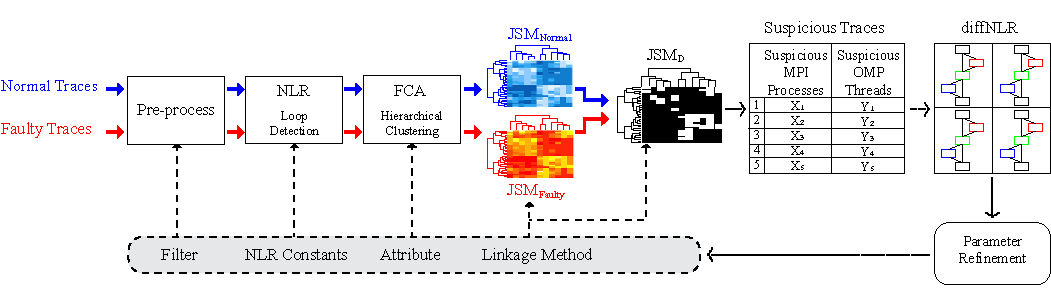
\includegraphics[width=1\textwidth]{diffTrace/figs/overview4.pdf}
\caption{DiffTrace overview}
%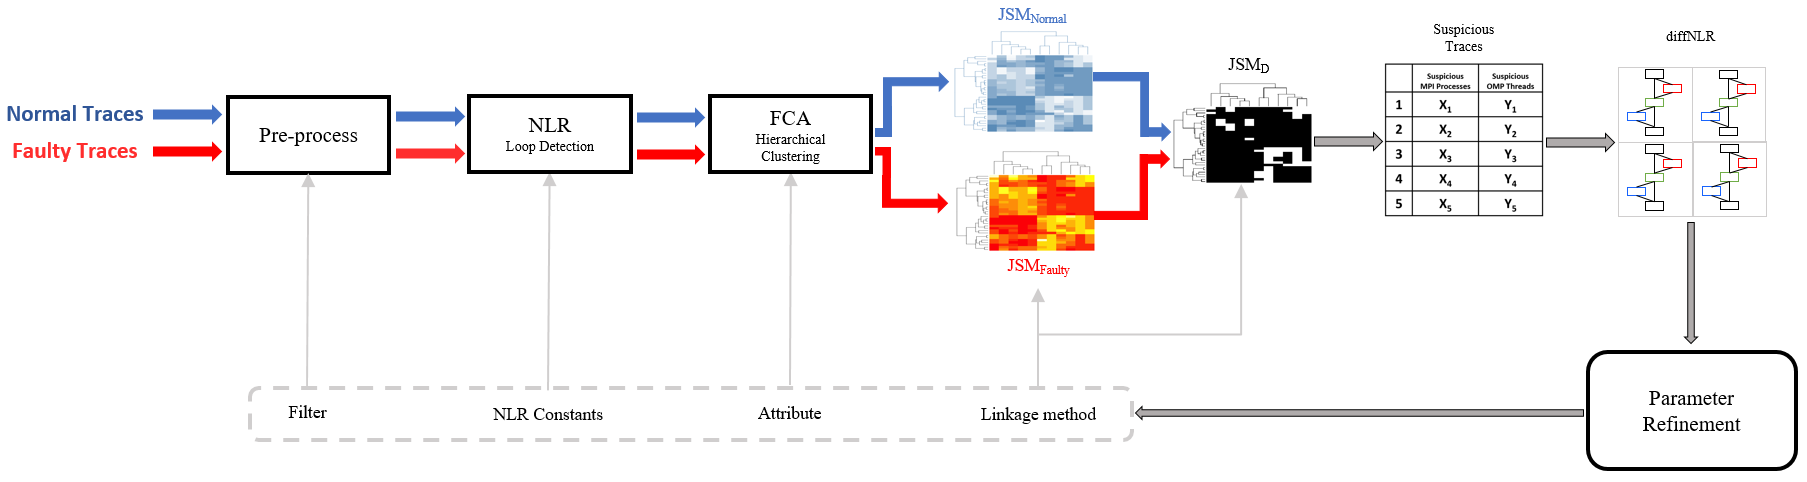
\includegraphics[]{figs/overview.png}
%\includegraphics[]{figs/overv}
\label{fig.diffTraceOverview}
\end{figure}


\begin{figure}[]
\centering
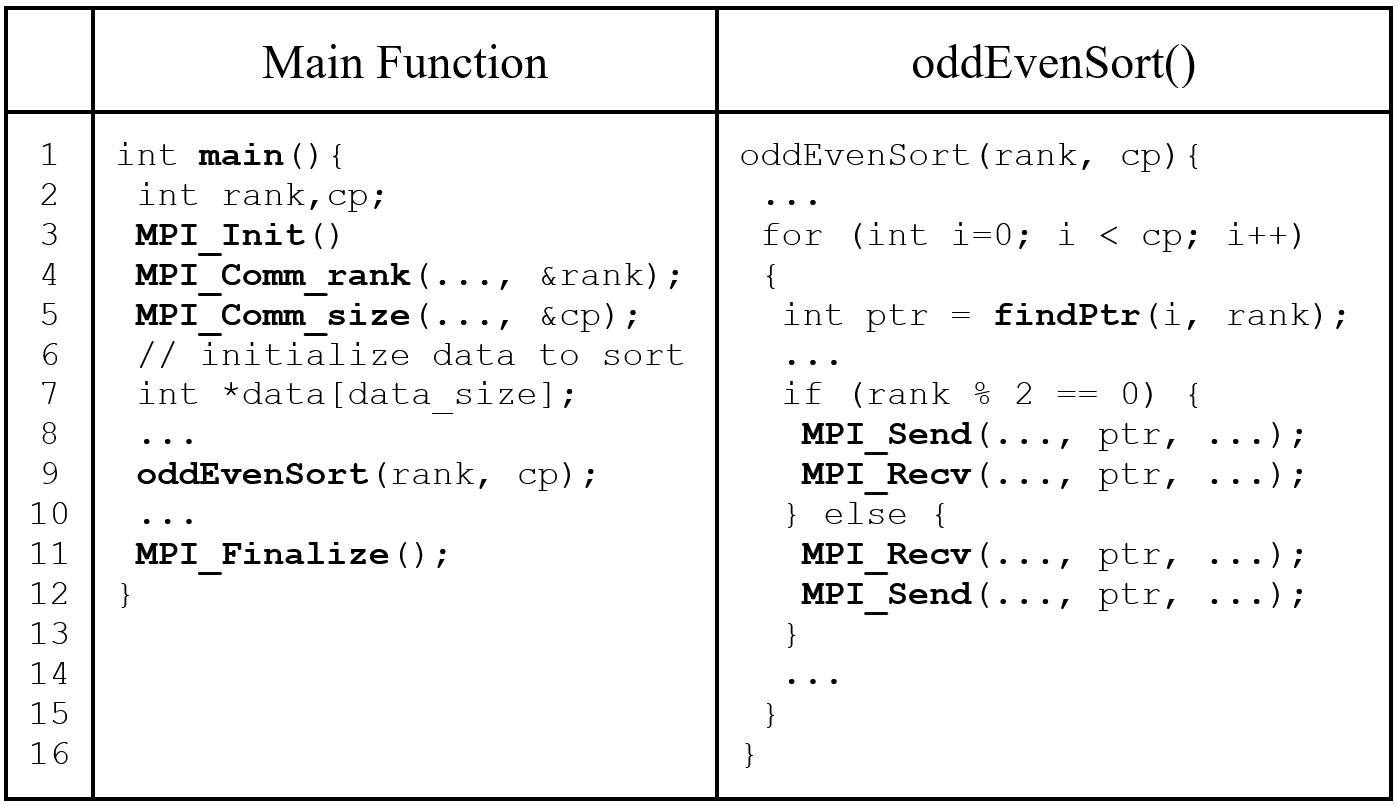
\includegraphics[width=.8\textwidth]{diffTrace/figs/oddEven.png}
\caption{Simplified MPI implementation of Odd/Even Sort}
\label{fig.oddEven}
\end{figure}

% Please add the following required packages to your document preamble:
% \usepackage{multirow}
\begin{table}[]
\centering
\caption{Predefined filters}
\label{tab:filters}
\scalebox{0.72}{
\begin{tabular}{|c|c|l|}
\hline
\textbf{Category} & \textbf{Sub-Category} & \multicolumn{1}{c|}{\textbf{Description}} \\ \hline
\multirow{2}{*}{Primary} & Returns & Filter out all returns \\ \cline{2-3}
 & PLT & \begin{tabular}[c]{@{}l@{}}Filter out the ".plt" function calls for external functions/procedures that \\ their address needs to be resolved dynamically from Procedure Linkage \\ Table (PLT)\end{tabular} \\ \hline
\multirow{4}{*}{MPI} & MPI All & Only keep functions that start with "MPI\_" \\ \cline{2-3}
 & MPI Collectives & Only keep MPI collective calls (MPI\_Barrier, MPI\_Allreduce, etc) \\ \cline{2-3}
 & MPI Send/Recv & Only keep MPI\_Send, MPI\_Isend, MPI\_Recv, MPI\_Irecv and MPI\_Wait \\ \cline{2-3}
 & MPI Internal Library & Keep all inner MPI library calls \\ \hline
\multirow{3}{*}{OMP} & OMP All & Only keep OMP calls (starting with GOMP\_) \\ \cline{2-3}
 & OMP Critical & Only keep OMP\_CRITICAL\_START and OMP\_CRITICAL\_END \\ \cline{2-3}
 & OMP Mutex & Only keep OMP\_Mutex calls \\ \hline
\multirow{4}{*}{System} & Memory & Keep any memory related functions (memcpy, memchk, alloc, malloc, etc) \\ \cline{2-3}
 & Network & Keep any network related functions (network, tcp, sched, etc) \\ \cline{2-3}
 & Poll & Keep any poll related functions (poll, yield, sched, etc) \\ \cline{2-3}
 & String & Keep any string related functions (strlen, strcpy, etc) \\ \hline
\multirow{2}{*}{Advanced} & Custom & Any regular expression can be captured \\ \cline{2-3}
 & Everything & Does not filter anything \\ \hline
\end{tabular}}
\end{table}


\begin{table}[]
\centering
\caption{The generated traces for odd/even execution with four processes}
\label{tab:oddEvenPT}
\scalebox{0.75}{
\begin{tabular}{|l|l|l|l|}
\hline
\rowcolor[HTML]{EFEFEF}
\multicolumn{1}{|c|}{\cellcolor[HTML]{EFEFEF}\textbf{$T_0$}} & \multicolumn{1}{c|}{\cellcolor[HTML]{EFEFEF}\textbf{$T_1$}} & \multicolumn{1}{c|}{\cellcolor[HTML]{EFEFEF}\textbf{$T_2$}} & \multicolumn{1}{c|}{\cellcolor[HTML]{EFEFEF}\textbf{$T_3$}} \\ \hline
... & ... & ... & ... \\ \\[-1em]  \hline
main & main & main & main \\ \\[-1em]  \hline
MPI\_Init & MPI\_Init & MPI\_Init & MPI\_Init \\ \\[-1em]  \hline
MPI\_Comm\_Rank & MPI\_Comm\_Rank & MPI\_Comm\_Rank & MPI\_Comm\_Rank \\ \\[-1em]  \hline
MPI\_Comm\_Size & MPI\_Comm\_Size & MPI\_Comm\_Size & MPI\_Comm\_Size \\ \\[-1em]  \hline
... & ... & ... & ... \\ \\[-1em]  \hline
oddEvenSort & oddEvenSort & oddEvenSort & oddEvenSort \\ \\[-1em]  \hline
... & ... & ... & ... \\ \\[-1em] \hline
findPtr & findPtr & findPtr & findPtr \\ \hline
\rowcolor[HTML]{FFCCC9}
{\color[HTML]{333333} MPI\_Send} & \cellcolor[HTML]{CBCEFB}{\color[HTML]{333333} MPI\_Recv} & {\color[HTML]{333333} MPI\_Send} & \cellcolor[HTML]{CBCEFB}{\color[HTML]{333333} MPI\_Recv} \\ \hline
\rowcolor[HTML]{FFCCC9}
{\color[HTML]{333333} MPI\_Recv} & \cellcolor[HTML]{CBCEFB}{\color[HTML]{333333} MPI\_Send} & {\color[HTML]{333333} MPI\_Recv} & \cellcolor[HTML]{CBCEFB}{\color[HTML]{333333} MPI\_Send} \\ \hline
... & ... & ... & ... \\ \hline
findPtr & findPtr & findPtr & findPtr \\ \hline
\rowcolor[HTML]{FFCCC9}
{\color[HTML]{333333} MPI\_Send} & \cellcolor[HTML]{CBCEFB}{\color[HTML]{333333} MPI\_Recv} & {\color[HTML]{333333} MPI\_Send} & \cellcolor[HTML]{CBCEFB}{\color[HTML]{333333} MPI\_Recv} \\ \hline
\rowcolor[HTML]{FFCCC9}
{\color[HTML]{333333} MPI\_Recv} & \cellcolor[HTML]{CBCEFB}{\color[HTML]{333333} MPI\_Send} & {\color[HTML]{333333} MPI\_Recv} & \cellcolor[HTML]{CBCEFB}{\color[HTML]{333333} MPI\_Send} \\ \hline
... & ... & ... & ... \\ \hline
MPI\_Finalize & MPI\_Finalize & MPI\_Finalize & MPI\_Finalize \\ \hline
\end{tabular}}
\end{table}


\begin{table}[]
\centering
\caption{NLR of traces}
\label{tab:oddEvenPT-NLR}
\scalebox{0.75}{
\begin{tabular}{|l|l|l|l|}
\hline
\rowcolor[HTML]{EFEFEF}
\multicolumn{1}{|c|}{\cellcolor[HTML]{EFEFEF}\textbf{$T_0$}} & \multicolumn{1}{c|}{\cellcolor[HTML]{EFEFEF}\textbf{$T_1$}} & \multicolumn{1}{c|}{\cellcolor[HTML]{EFEFEF}\textbf{$T_2$}} & \multicolumn{1}{c|}{\cellcolor[HTML]{EFEFEF}\textbf{$T_3$}} \\ \hline
MPI\_Init & MPI\_Init & MPI\_Init & MPI\_Init \\ \\[-1em]  \hline
MPI\_Comm\_Rank & MPI\_Comm\_Rank & MPI\_Comm\_Rank & MPI\_Comm\_Rank \\ \\[-1em]  \hline
MPI\_Comm\_Size & MPI\_Comm\_Size & MPI\_Comm\_Size & MPI\_Comm\_Size \\ \\[-1em]  \hline
\rowcolor[HTML]{FFCCC9}
{\color[HTML]{333333} L0 \^{} 2} & \cellcolor[HTML]{CBCEFB}{\color[HTML]{333333} L1 \^{} 4} & {\color[HTML]{333333} L0 \^{} 4} & \cellcolor[HTML]{CBCEFB}{\color[HTML]{333333} L1 \^{} 2} \\ \hline
MPI\_Finalize & MPI\_Finalize & MPI\_Finalize & MPI\_Finalize \\ \hline
\end{tabular}}
\end{table}





\begin{small}
\begin{algorithm}[]
 \DontPrintSemicolon
 \SetKwFunction{KwReduce}{Reduce}
% \SetKwInOut{Input}{Input} \SetKwInOut{Output}{Output}\SetKwInOut{Local}{Local}
  %\SetKw{KwEach}{each}
 %\Input{Stack of elements $S$, $S[1]$ is top}
 %\Output{$NLR(T)$}
 \KwReduce{$S$}:{\\
 \Indp
     \For{$ i:1$ ... $3K$}{
         $b$ = $i/3$\;
         \If{Top 3 $b$-long elements of $S$ are \textit{isomorphic}}{
             pop $i$ elements from $S$\;
             $LB=S[b:1]$,
             $LC=3$\;
             $LS=(LB,LC)$\;
             push $LS$ to $S$\;
             add $LB$ to the Loop Table\;
             \KwReduce{$S$}\;
         }
         \If{ $S[i]$ is a loop ($LS$) and $S[i-1:1]$ isomorphic to its loop body$LB$}{
             $LC=LC+1$\;
             pop $i-1$ elements from $S$\;
             \KwReduce{$S$}\;
         }
     }
 }

 \caption{\texttt{Reduce} procedure adapted from the NLR algorithm }
 \label{proc:NLR}
\end{algorithm}
\end{small}



\begin{table}[]
\caption{Formal Context of odd/even sort example}
\label{tab:sampleContext}
\scalebox{0.7}{
\begin{tabular}{l|cccccc}
 & \multicolumn{1}{l}{MPI\_Init()} & \multicolumn{1}{l}{MPI\_Comm\_Size()} & \multicolumn{1}{l}{MPI\_Comm\_Rank()} & \multicolumn{1}{l}{L0} & \multicolumn{1}{l}{L1} & \multicolumn{1}{l}{MPI\_Finalize()} \\ \hline
Trace 0 & $\times$ & $\times$ & $\times$ & $\times$ &  & $\times$ \\
Trace 1 & $\times$ & $\times$ & $\times$ &  & $\times$ & $\times$ \\
Trace 2 & $\times$ & $\times$ & $\times$ & $\times$ &  & $\times$ \\
Trace 3 & $\times$ & $\times$ & $\times$ &  & $\times$ & $\times$
\end{tabular}}
\end{table}



% Please add the following required packages to your document preamble:
% \usepackage{multirow}
\begin{table}[]
\caption{Attributes mined from traces}
\label{tab:atr}
\centering
\scalebox{0.9}{
\begin{tabular}{|l|l|c|l|}
\hline
\multicolumn{4}{|c|}{\begin{tabular}[c]{@{}c@{}}\textbf{Attributes}\\ \{attr:freq\}\end{tabular}} \\ \hline
\multicolumn{2}{|c|}{attr} & \multicolumn{2}{c|}{freq} \\ \hline
\multirow{3}{*}{\textbf{Single}} & \multirow{3}{*}{\begin{tabular}[c]{@{}l@{}}each entry \\ of the trace\end{tabular}} & \multirow{2}{*}{\textbf{Actual}} & \multirow{2}{*}{observed frequency} \\
 &  &  &  \\ \cline{3-4} 
 &  & \multirow{2}{*}{\textbf{Log10}} & \multirow{2}{*}{log10 of the observed frequency} \\ \cline{1-2}
\multirow{3}{*}{\textbf{Double}} & \multirow{3}{*}{\begin{tabular}[c]{@{}l@{}}each pair of \\ consecutive entries\end{tabular}} &  &  \\ \cline{3-4} 
 &  & \multirow{2}{*}{\textbf{noFreq}} & \multirow{2}{*}{no frequency} \\
 &  &  &  \\ \hline
\end{tabular}}
\end{table}



\begin{figure}[]
\centering
  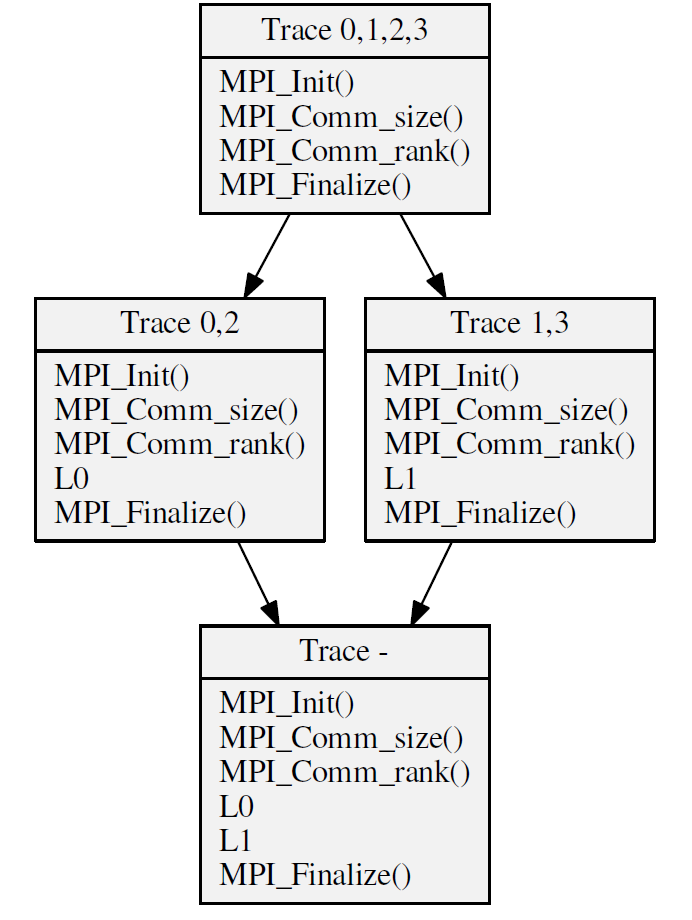
\includegraphics[width=.55\textwidth]{diffTrace/figs/sampleCL.png}
  \caption{Sample concept lattice from object-attribute context in Table \ref{tab:sampleContext}}
  \label{fig:sampleCL}
\end{figure}

\begin{figure}[]
\centering
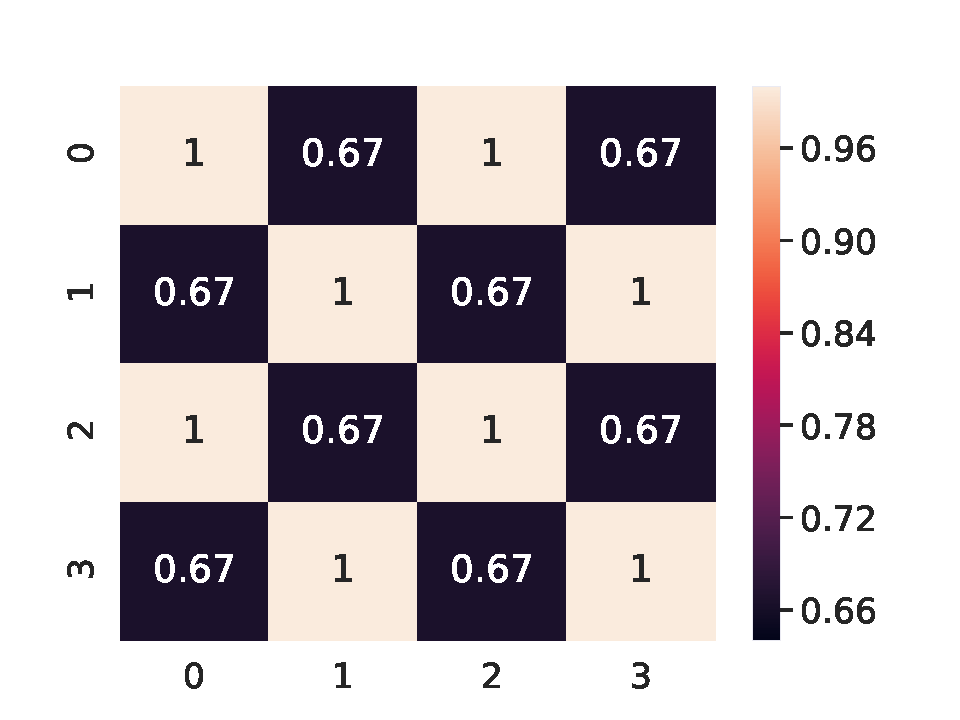
\includegraphics[width=.4\textwidth]{diffTrace/figs/oddEvenJSM2.pdf}
\caption{Pairwise Jaccard Similarity Matrix (JSM) of MPI processes in sample code}
\label{fig:jsm2}
\end{figure}




\begin{figure}[]
    \centering
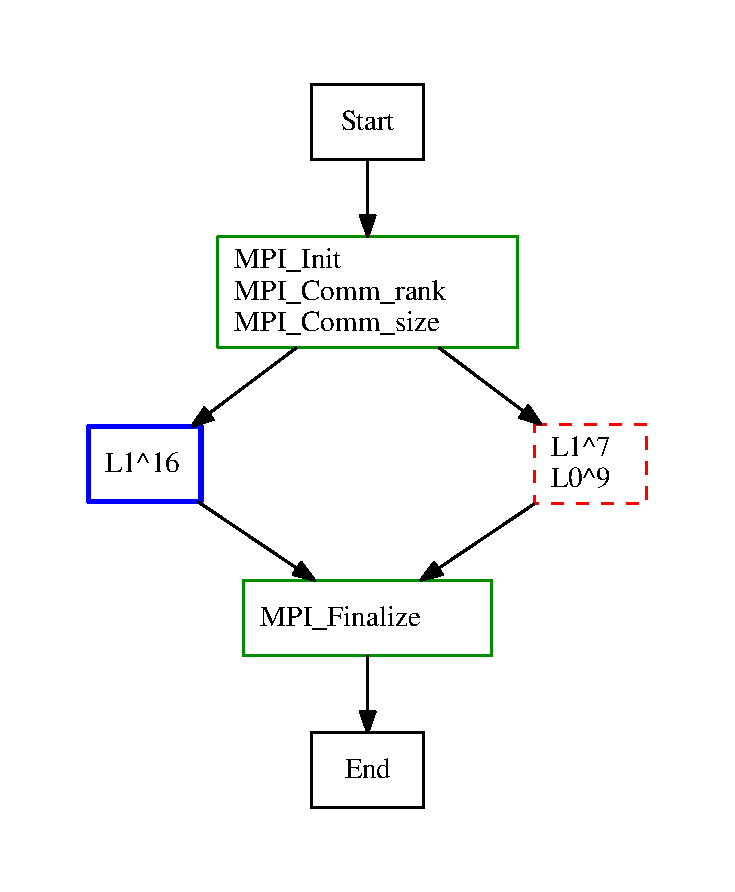
\includegraphics[width=.6\textwidth]{diffTrace/figs/b-11.mpi.0K10-5.pdf}
\caption{swapBug}
\label{fig:swapbug}
\end{figure}
%\caption{diffNLR Example}
%\label{fig:sampleDiffNLR}
\begin{figure}[]
\centering
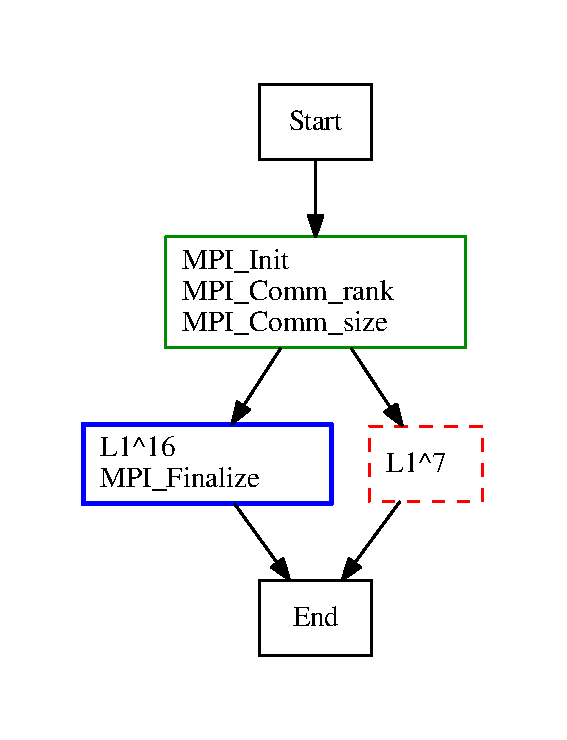
\includegraphics[width=.6\linewidth]{diffTrace/figs/adl-11.mpi.0K10-5.pdf}
\caption{dlBug}
\label{fig:dlbug}
\end{figure}

\begin{figure}[]
\centering
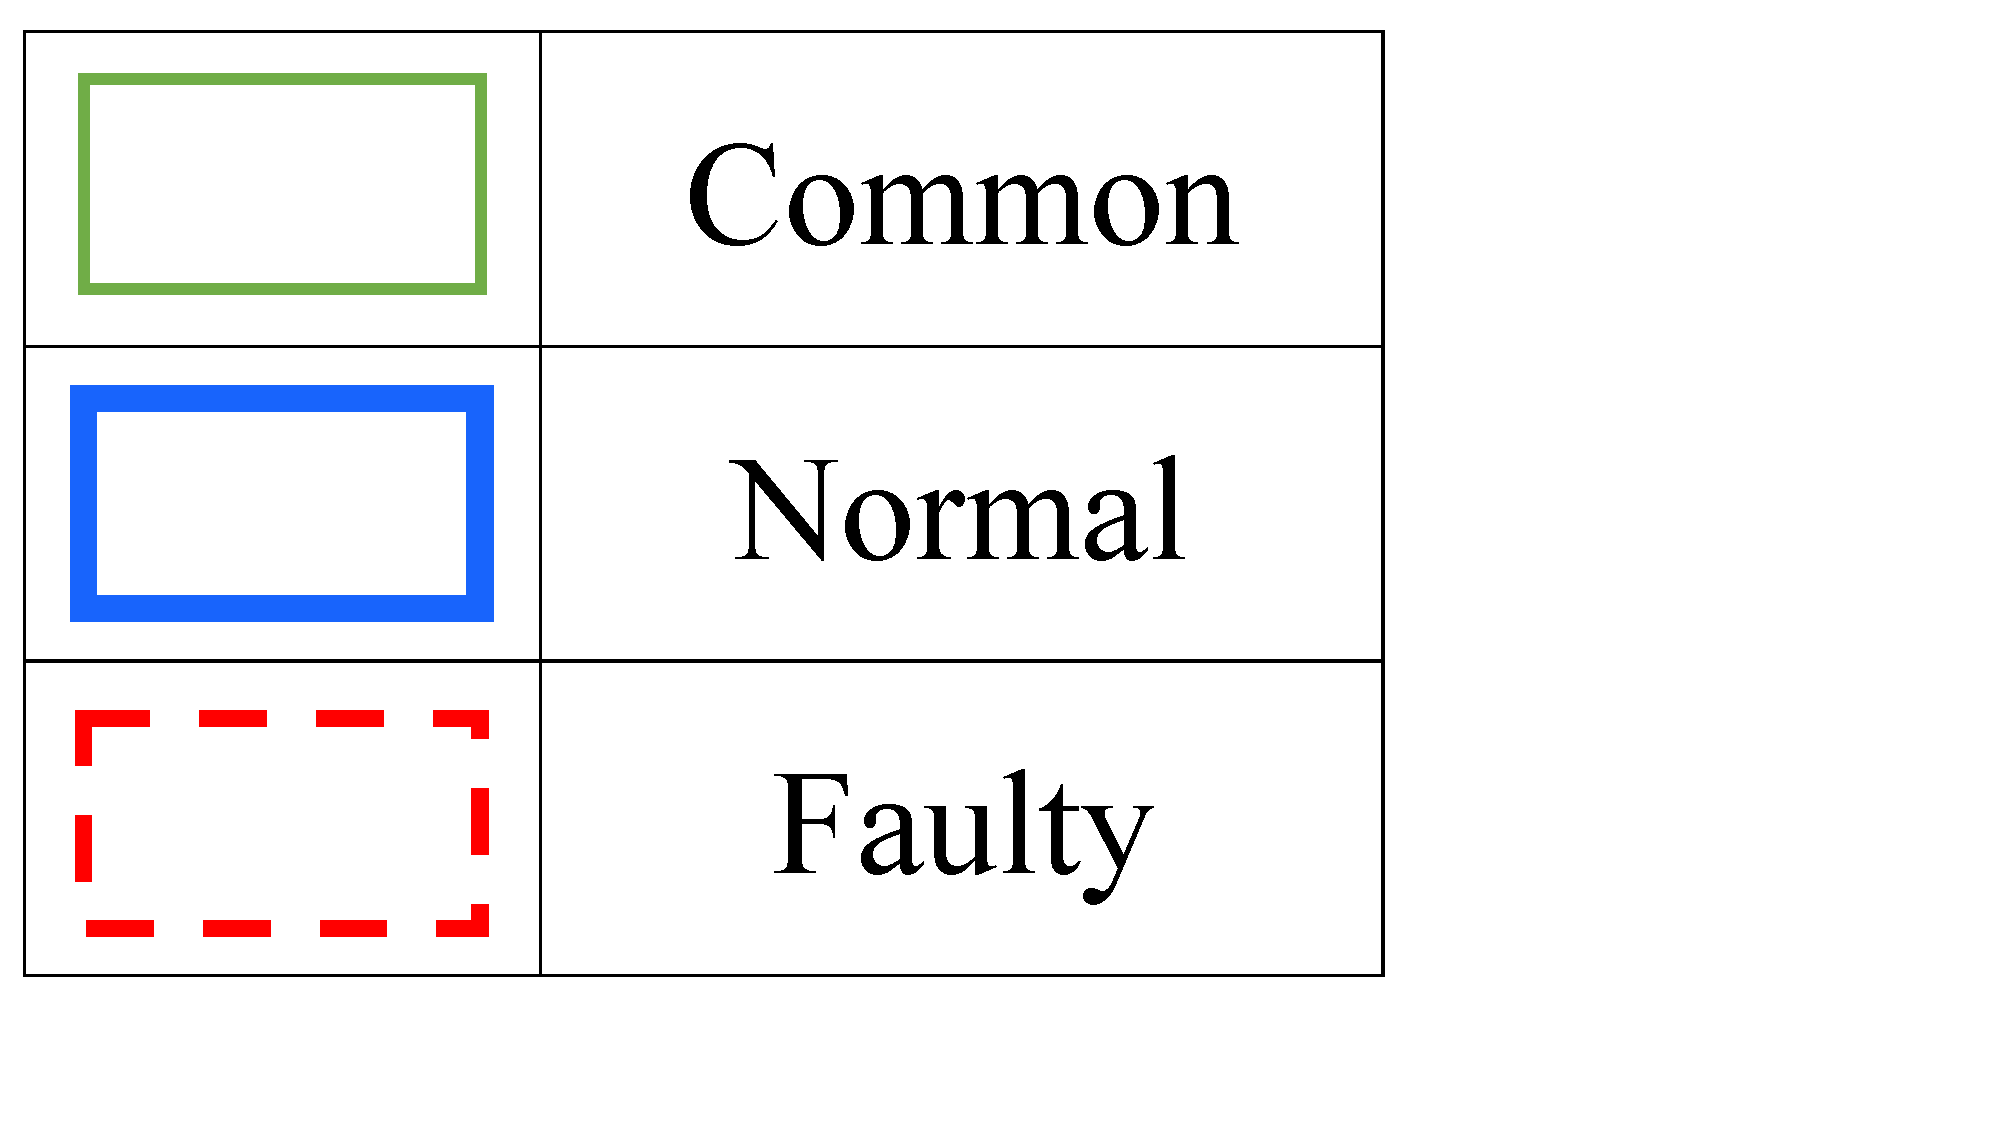
\includegraphics[width=.2\textwidth]{diffTrace/figs/legend.pdf}
\caption{Legend}
\label{fig:legend}
\end{figure}



\begin{table}[t]
\centering
\caption{Ranking table - OpenMP bug: unprotected shared memory access by thread 4 of process 6}
\label{tab:mc1-mc-6-4}
\scalebox{0.78}{
\begin{tabular}{|c|c|c|c|c|}
\hline
 Filter                           & Attributes   &   B-score & \begin{tabular}[c]{@{}c@{}}Top\\Processes\end{tabular}          & \begin{tabular}[c]{@{}c@{}}Top\\Threads\end{tabular}  \\
\hline
 11.plt.mem.cust.0K10             & doub.noFreq  &     0.244 & 7, 3, 4         & \textbf{6.4}, 7.3, 1.4, 3.3, 3.4, 4.2  \\
 11.plt.mem.cust.0K10             & doub.log10   &     0.244 & 7, 3, 4         & \textbf{6.4}, 7.3, 1.4, 3.3, 3.4, 4.2  \\
 01.plt.mem.cust.0K10             & doub.noFreq  &     0.244 & 7, 3, 4         & \textbf{6.4}, 7.3, 1.4, 3.3, 3.4, 4.2  \\
 01.plt.mem.cust.0K10             & doub.log10   &     0.244 & 7, 3, 4         & \textbf{6.4}, 7.3, 1.4, 3.3, 3.4, 4.2  \\
 01.mem.ompcrit.cust.0K10         & sing.log10   &     0.262 & 3                 & \textbf{6.4}, 7.1, 3.3, 4.1, 5.1, 6.1  \\
 01.mem.ompcrit.cust.0K10         & sing.noFreq  &     0.262 & 3                 & \textbf{6.4}, 7.1, 3.3, 4.1, 5.1, 6.1  \\
 11.mem.ompcrit.cust.0K10         & sing.log10   &     0.262 & 3                 & \textbf{6.4}, 7.1, 3.3, 4.1, 5.1, 6.1  \\
 11.mem.ompcrit.cust.0K10         & sing.noFreq  &     0.262 & 3                 & \textbf{6.4}, 7.1, 3.3, 4.1, 5.1, 6.1  \\
% 01.plt.mem.mpi.ompall.cust.0K10  & sing.actual  &     0.266 &                    & 2.4 , 4.3 ,                         \\
% 11.plt.mem.mpi.ompall.cust.0K10  & sing.actual  &     0.266 &                    & 2.4 , 4.3 ,                         \\
 11.plt.mem.cust.0K10             & doub.actual  &     0.273 & 7                 & \textbf{6.4}, 2.4, 3.4, 4.2, 4.4        \\
 01.plt.mem.cust.0K10             & doub.actual  &     0.273 & 7                 & \textbf{6.4}, 2.4, 3.4, 4.2, 4.4        \\
% 11.plt.mem.mpi.ompcrit.cust.0K10 & doub.noFreq  &     0.276 & 3 ,                & 3.3 , \textbf{6.4} ,                         \\
% 11.plt.mem.mpi.ompcrit.cust.0K10 & doub.log10   &     0.276 & 3 ,                & 3.3 , \textbf{6.4} ,                         \\
% 01.plt.mem.mpi.ompcrit.cust.0K10 & doub.noFreq  &     0.276 & 3 ,                & 3.3 , \textbf{6.4} ,                         \\
% 01.plt.mem.mpi.ompcrit.cust.0K10 & doub.log10   &     0.276 & 3 ,                & 3.3 , \textbf{6.4} ,                         \\
\hline
\end{tabular}}
\end{table}


\begin{table}[b]
\centering
\caption{Ranking table - MPI bug: wrong collective size in process 2}
\label{tab:ar1-ws-all-nn}
\scalebox{0.81}{
\begin{tabular}{|c|c|c|c|c|}
\hline
 Filter              & Attributes   &    B-score & \begin{tabular}[c]{@{}c@{}}Top\\Processes\end{tabular}          & \begin{tabular}[c]{@{}c@{}}Top\\Threads\end{tabular}         \\
\hline
% 11.mem.mpicol.ompcrit.cust.0K10 & sing.log10   &      0.383 & 0 , 7 , 2 , 4 , 5 , 6 , & 1.1 , 1.3 , 1.4 , 3.1 , 3.2 , 3.4 , \\
% 11.mem.mpicol.ompcrit.cust.0K10 & sing.noFreq  &      0.383 & 0 , 7 , 2 , 4 , 5 , 6 , & 1.1 , 1.3 , 1.4 , 3.1 , 3.2 , 3.4 , \\
 11.mpicol.cust.0K10             & sing.log10   &      0.439 & 0, 7, 2, 4, 5, 6  & 1.1, 1.3, 3.1, 3.2, 3.4        \\
 11.mpicol.cust.0K10             & sing.noFreq  &      0.439 & 0, 7, 2, 4, 5, 6  & 1.1, 1.3, 3.1, 3.2, 3.4        \\
 11.mpi.cust.0K10                & doub.noFreq  &      0.457 & 0, 7, 2, 4, 5, 6  & 1.4, 3.3, 3.4                    \\
 11.mpi.cust.0K10                & doub.actual  &      0.457 & 0, 7, 2, 4, 5, 6  & 1.4, 3.3, 3.4                    \\
 11.mpiall.cust.0K10             & doub.noFreq  &      0.457 & 0, 7, 2, 4, 5, 6  & 1.4, 3.3, 3.4                    \\
 11.mpiall.cust.0K10             & doub.actual  &      0.457 & 0, 7, 2, 4, 5, 6  & 1.4, 3.3, 3.4                    \\
 11.mpicol.cust.0K10             & doub.noFreq  &      0.457 & 0, 7, 2, 4, 5, 6  & 1.4, 3.3, 3.4                    \\
 11.mpicol.cust.0K10             & doub.actual  &      0.457 & 0, 7, 2, 4, 5, 6  & 1.4, 3.3, 3.4                    \\
 11.mpi.cust.0K10                & sing.log10   &      0.465 & 0, 7, 2, 4, 5, 6  & 1.1, 1.3, 3.1, 3.2, 3.4        \\
 11.mpi.cust.0K10                & sing.noFreq  &      0.465 & 0, 7, 2, 4, 5, 6  & 1.1, 1.3, 3.1, 3.2, 3.4        \\
 11.mpiall.cust.0K10             & sing.log10   &      0.465 & 0, 7, 2, 4, 5, 6  & 1.1, 1.3, 3.1, 3.2, 3.4        \\
 11.mpiall.cust.0K10             & sing.noFreq  &      0.465 & 0, 7, 2, 4, 5, 6  & 1.1, 1.3, 3.1, 3.2, 3.4        \\
 11.mpi.cust.0K10                & doub.noFreq  &      0.543 & 0, 7, 2, 4, 5, 6  & 1.4, 3.3, 3.4                    \\
 11.mpi.cust.0K10                & doub.actual  &      0.543 & 0, 7, 2, 4, 5, 6  & 1.4, 3.3, 3.4                    \\
\hline
\end{tabular}}
\end{table}

\newpage
\begin{frame}{}
  \lstset{language=C}
 \begin{lstlisting}[caption={ILCS Overview},label={lst:ilcs}]
main(argc, argv) {
 ... // initialization
 MPI_Init();
 MPI_Comm_size();
 MPI_Comm_rank(my_rank);
 ... // Obtain number of local CPUs and GPUs
 MPI_Reduce(lCPUs, gCPUs, MPI_SUM); // Total # of CPUs
 MPI_Reduce(lGPUs, gGPUs, MPI_SUM); // Total # of GPUs
 champSize = CPU_Init();
 ... // Memory allocation for storing local and global champions w.r.t. champSize
 MPI_Barrier();
 <@\textcolor{blue} {\#pragma omp parallel num\_threads(lCPUs+1)}@>
 {rank = omp_get_thread_num();
  if (rank != 0) { // worker threads
   while (cont) {
    ... // calculate seed
    local_result = CPU_Exec();
    if (local_result < champ[rank]) { // update local champion
     <@\textcolor{blue}{\#pragma omp critical}@>
     memcpy(champ[rank], local_result);}}
  } else { //master thread
   do {
    ...
    MPI_AllReduce(); //broadcast the global champion 
	  ...
    MPI_AllReduce(); //broadcast the global champion P_id
    ...
    if (my_rank == global_champion_P_id) {
     <@\textcolor{blue}{\#pragma omp critical}@>
     memcpy(bcast_buffer, champ[rank]);
    }
    MPI_Bcast(bcast_buffer); // broadcast the local champion to all nodes
   } while (no_change_threshold);
   cont = 0; // signal worker threads to terminate
  }}
 if (my_rank == 0) {CPU_Output(champ);}
 MPI_Finalize();}

/* User code for TSP problem */
CPU_Init() {/* Read coordinates, calculate distances, initialize champion structure, return structure size */}
CPU_Exec() {/* Find local champions (TSP tours) */}
CPU_Output() {/* Output champion */}
\end{lstlisting}
\end{frame}

\newpage
\begin{table}[b]
\centering
\caption{Ranking Table - MPI-Bug: Wrong Collective Operation ,Injected to Process 0}
\label{tab:ar1-wo-0-nn}
\scalebox{0.81}{
\begin{tabular}{|c|c|c|c|c|}
\hline
 Filter              & Attributes   &    B-score & \begin{tabular}[c]{@{}c@{}}Top\\Processes\end{tabular}          & \begin{tabular}[c]{@{}c@{}}Top\\Threads\end{tabular}  \\
\hline
 01.plt.cust.0K10    & doub.log10   &      0.271 & 2                 & 6.2, 7.3, 2.2, 5.2, 5.3  \\
 11.plt.cust.0K10    & doub.log10   &      0.271 & 2                 & 6.2, 7.3, 2.2, 5.2, 5.3  \\
 01.plt.cust.0K10    & sing.actual  &      0.276 & 1                 & 3.1, 1.4, 6.4, 3.4        \\
 11.plt.cust.0K10    & sing.actual  &      0.276 & 1                 & 3.1, 1.4, 6.4, 3.4        \\
 01.plt.cust.0K10    & doub.noFreq  &      0.285 & 2                 & 6.2, 7.3, 2.2, 5.2, 5.3  \\
 11.plt.cust.0K10    & doub.noFreq  &      0.285 & 2                 & 6.2, 7.3, 2.2, 5.2, 5.3  \\
 01.plt.cust.0K10    & sing.log10   &      0.292 & 1, 4, 5  & 3.1, 4.3                    \\
 11.plt.cust.0K10    & sing.log10   &      0.292 & 1, 4, 5   & 3.1, 4.3                    \\
 01.\textbf{mpicol}.cust.0K10 & sing.actual  &      0.312 & \textbf{5}                 & 3.2, 6.4, 5.4, 4.2        \\
 11.\textbf{mpicol}.cust.0K10 & sing.actual  &      0.312 & \textbf{5}                 & 3.2, 6.4, 5.4, 4.2        \\
 11.\textbf{mpi}.cust.0K10    & sing.actual  &      0.331 & \textbf{5}                 & 3.2, 6.4, 5.4, 4.2        \\
 11.\textbf{mpiall}.cust.0K10 & sing.actual  &      0.331 & \textbf{5}                 & 3.2, 6.4, 5.4, 4.2        \\
 01.\textbf{mpiall}.cust.0K10 & sing.actual  &      0.331 & \textbf{5}                 & 3.2, 6.4, 5.4, 4.2        \\
 01.\textbf{mpi}.cust.0K10    & sing.actual  &      0.331 & \textbf{5}                 & 3.2, 6.4, 5.4, 4.2        \\
 11.\textbf{mpi}.cust.0K10    & sing.actual  &      0.371 & \textbf{5}                 & 3.2, 6.4, 5.4, 4.2        \\
 11.\textbf{mpiall}.cust.0K10 & sing.actual  &      0.371 & \textbf{5}                 & 3.2, 6.4, 5.4, 4.2        \\
\hline
\end{tabular}}
\end{table}



\begin{figure}[]
     \centering
     \begin{subfigure}[b]{0.31\textwidth}
        \centering
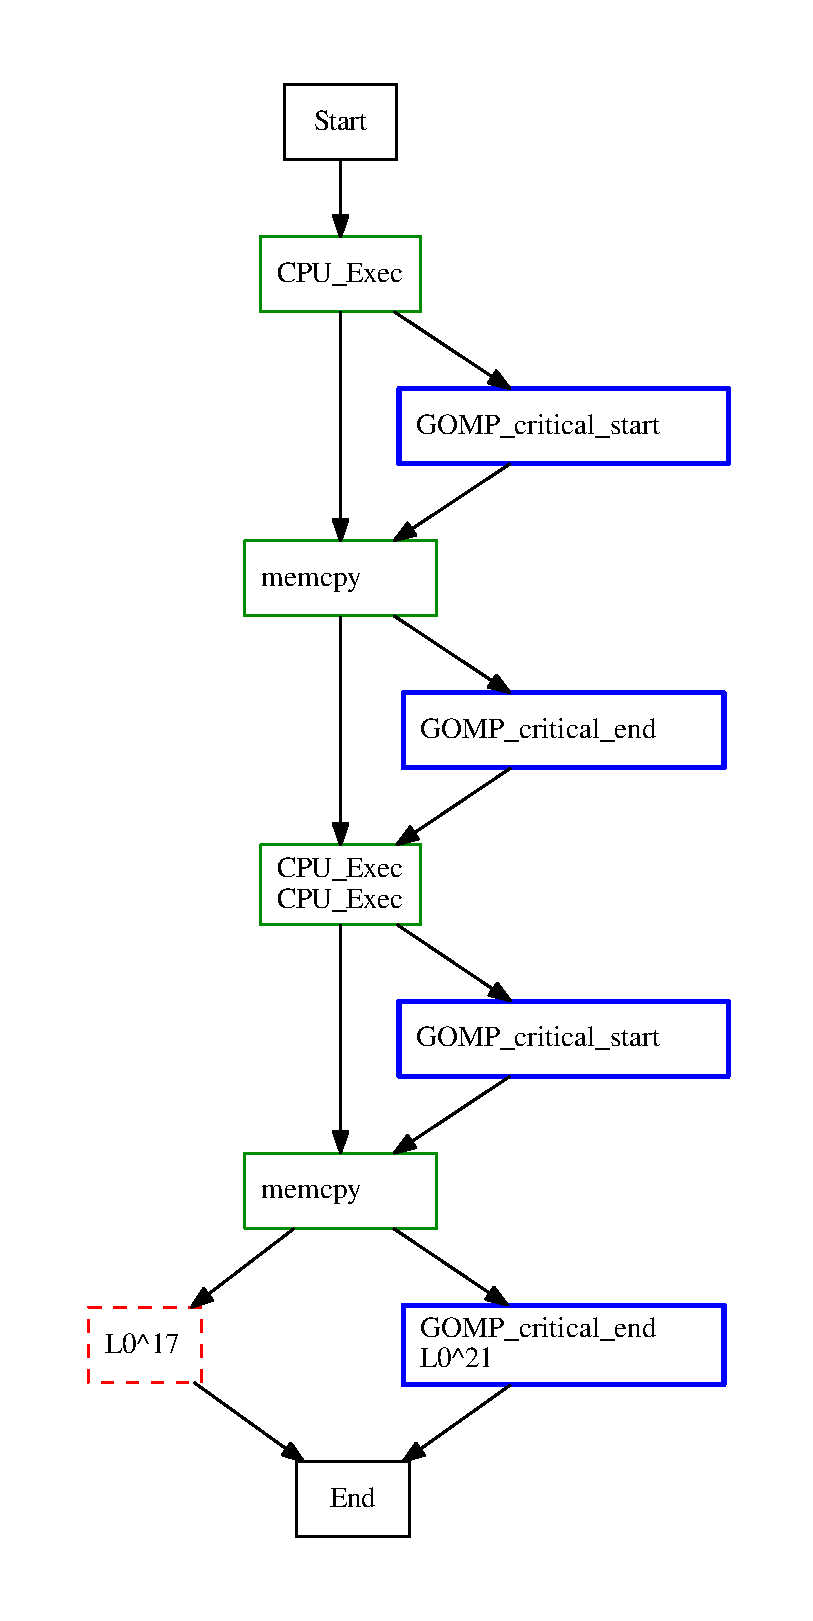
\includegraphics[width=\textwidth]{diffTrace/figs/diffNLR/ompBug-6-4-x0.pdf}
\caption{diffNLR(6.4)}
\label{diffNLR-6-4}
     \end{subfigure}
     \hfill
     \begin{subfigure}[b]{0.31\textwidth}
       \centering
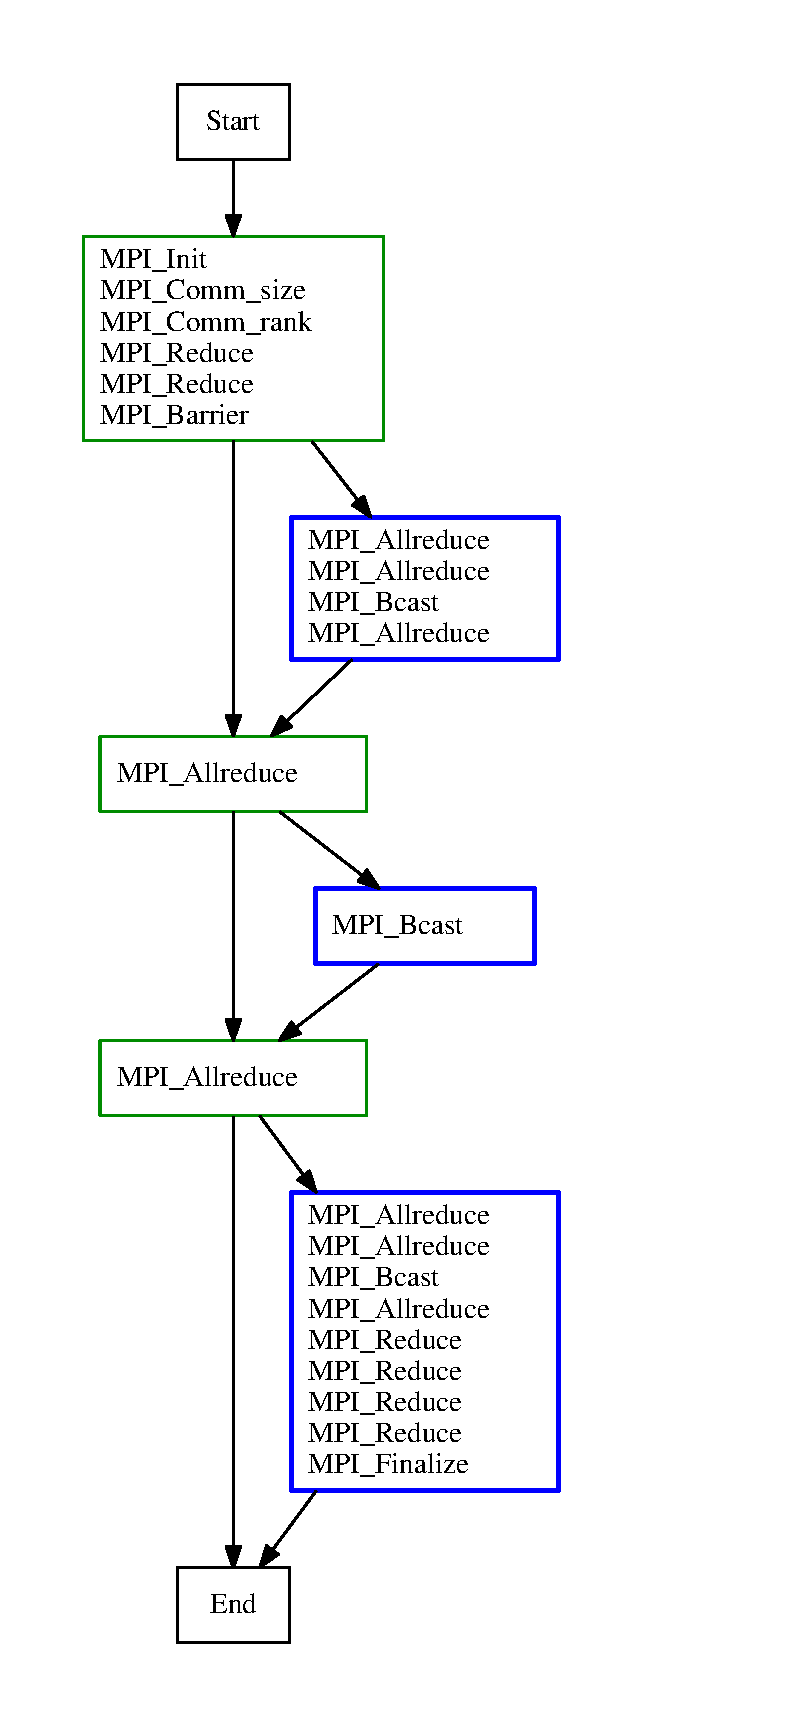
\includegraphics[width=\textwidth]{diffTrace/figs/diffNLR/mpiBug-all-nn-x0.pdf}
\caption{diffNLR(4)}
\label{diffNLR-0}
     \end{subfigure}
     \hfill
     \begin{subfigure}[b]{0.31\textwidth}
         \centering
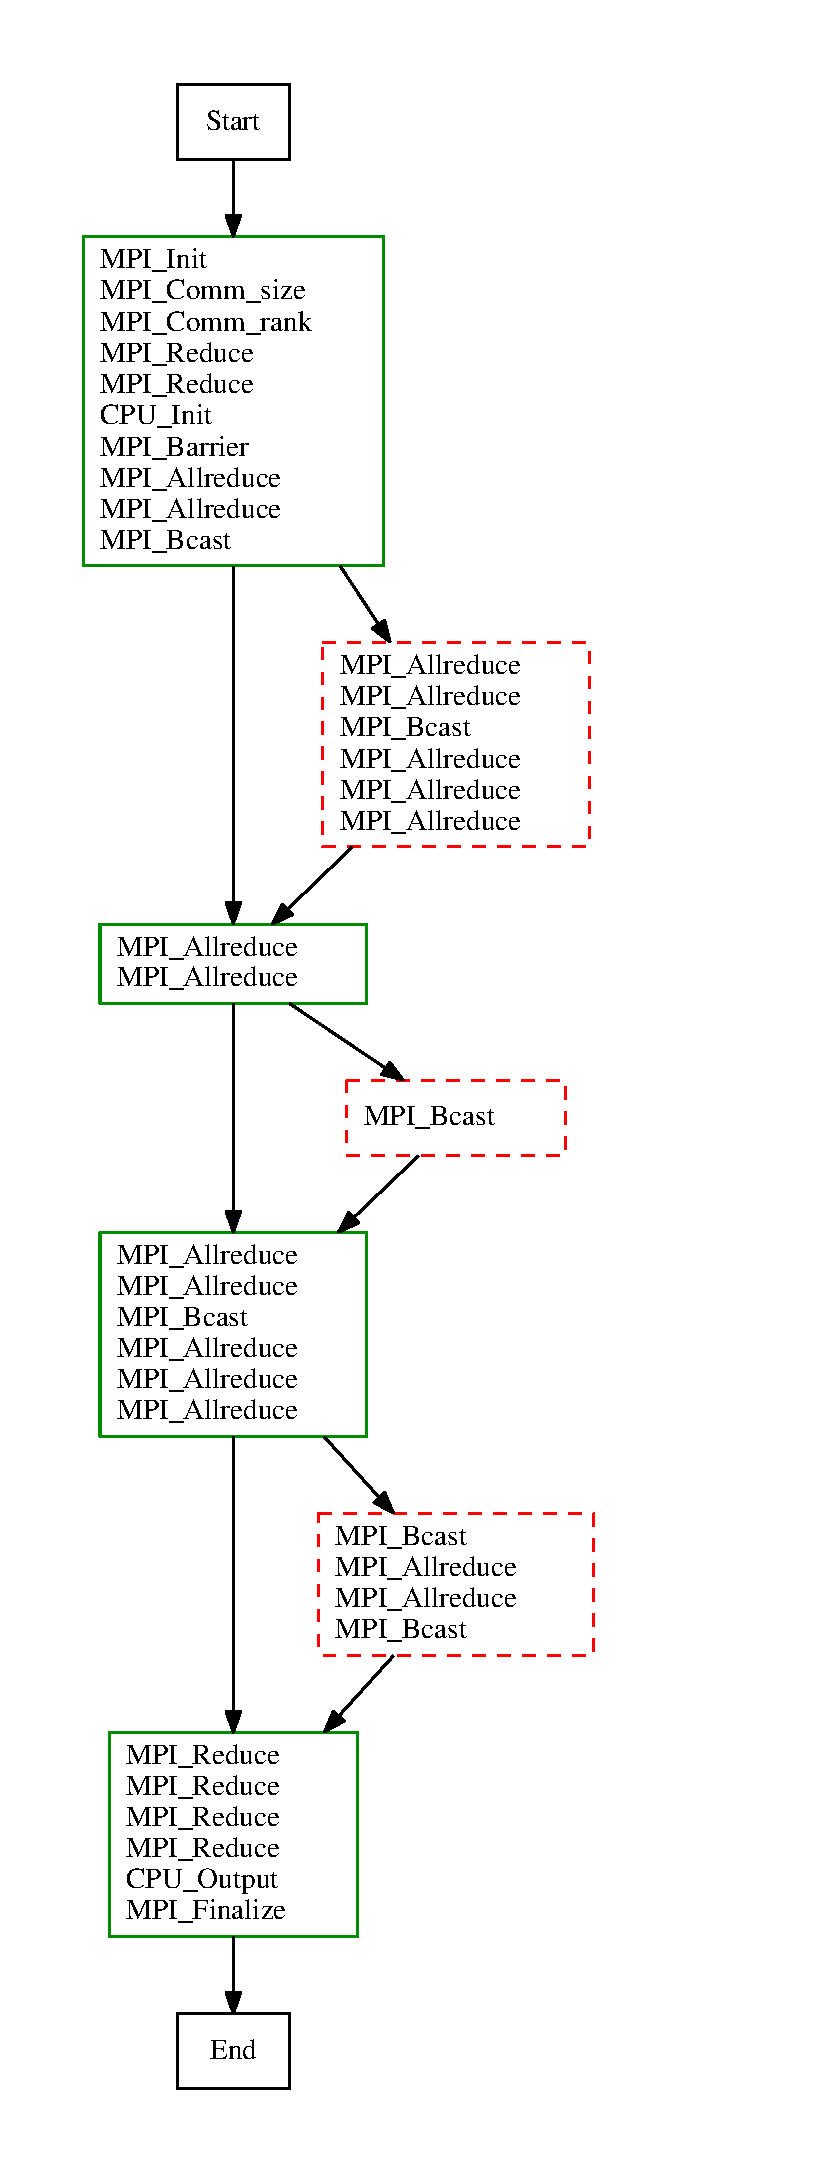
\includegraphics[width=0.9\textwidth]{diffTrace/figs/diffNLR/mpiBug2-0-nn-x0.pdf}
\caption{diffNLR(5)}
\label{diffNLR-5}
     \end{subfigure}
        \caption{Three diffNLR outputs}
        \label{fig:three graphs}
\end{figure}

\begin{table}[t]
\centering
\caption{Ranking Table for LULESH}
\label{tab:lulesh}
\scalebox{1.01}{
\begin{tabular}{|l|l|r|l|}
\hline
 Filter   & Attributes   &  B-score & Top Processes        \\
\hline
 11.1K10  & sing.noFreq  &    0.295 & \textbf{2} , 3 , 4 , 5 , 6 , 7   \\
 01.1K10  & sing.noFreq  &    0.354 & 0 , 1 , \textbf{2} , 3 , 4 , 5   \\
 01.1K10  & sing.actual  &    0.383 & \textbf{2} , 3 , 4 , 5 , 6 , 7   \\
 11.1K10  & sing.noFreq  &    0.408 & \textbf{2} , 3 , 4 , 5 , 6 , 7   \\
 11.1K10  & sing.noFreq  &    0.408 & \textbf{2} , 3 , 4 , 5 , 6 , 7   \\
 01.1K10  & doub.noFreq  &    0.433 & 4 , 5 , 6               \\
 01.1K10  & doub.noFreq  &    0.433 & 4 , 5 , 6               \\
 11.1K10  & doub.noFreq  &    0.433 & 5 , 1 , 6               \\
 01.1K10  & doub.noFreq  &    0.455 & 1 , \textbf{2} , 3 , 4 , 7       \\
 11.1K10  & doub.noFreq  &    0.458 & 5 , 1 , 6               \\
 11.1K10  & doub.noFreq  &    0.458 & 4 , 5 , 6 , 7           \\
 01.1K10  & sing.log10   &    0.459 & 1 , \textbf{2} , 3 , 4 , 5 , 6   \\
 01.1K10  & doub.noFreq  &    0.472 & 0 , 1 , \textbf{2} , 3 , 4 , 5   \\
 01.1K10  & sing.log10   &    0.475 & 1 , 3 , 4 , 5 , 6 , 7   \\
 01.1K10  & sing.log10   &    0.478 & 1 , \textbf{2} , 3 , 4 , 5 , 6   \\
 01.1K10  & sing.log10   &    0.478 & 1 , \textbf{2} , 3 , 4 , 5 , 6   \\
\hline
\end{tabular}}
\end{table}

